\begin{figure}[htb]
    \centering
    \resizebox{0.95\linewidth}{!}{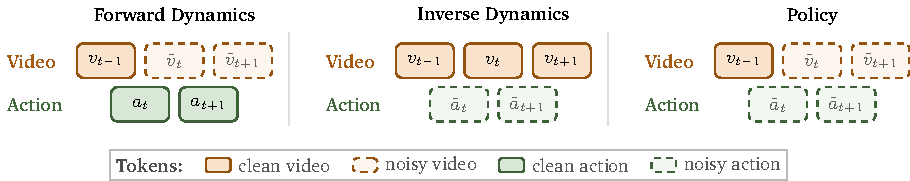
\includegraphics{figures/model_architecture/action/tikz_action_modes.pdf}}
    \caption{\textbf{Action sequence configurations.} For a video-action data sample, Cosmos 3 constructs different training modes by varying which tokens are clean and which are noisy. The diagram shows a local temporal window in which action tokens lie between adjacent video tokens: $\acttok_{t}$ connects $\vidtok_{t{-}1}$ to $\vidtok_{t}$, and $\acttok_{t{+}1}$ connects $\vidtok_{t}$ to $\vidtok_{t{+}1}$. Forward dynamics mode denoises vision tokens conditioned on clean action tokens; inverse dynamics mode denoises action tokens conditioned on clean vision tokens; and video-action (policy) mode denoises both vision and action tokens. Language and special tokens are omitted for compactness.}
    \label{fig:action_modes}
\end{figure}
